\documentclass[a4paper,12pt]{report}

\usepackage[utf8]{inputenc}
\usepackage[french]{babel}
\usepackage{graphicx}

\title{Metamorphe}
\author{NIOBE Cyril, GAITON Cyril, AMILCARO Simon, TOUDIC Anthony}
\date{\today}

\begin{document}
\maketitle
\tableofcontents
\setcounter{tocdepth}{5}

\chapter{Présentation du sujet}
Ce projet a pour but de simuler une anamorphose photographique à partir d’une séquences d’images tirée d’une vidéo.
Afin de bien comprendre le sujet, il nous a été présenté le fonctionnement d’un appareil photographique avec obturateur à rideaux puisque c’est avec ce mécanisme qu’en résulte une image anamorphosée.
Ce traitement d’images sera sous la forme d’une application Android codée en Java et donc exécuté avec les capacités d’un smartphone.\par\bigskip

Nous avons donc pour objectif d’extraire un nombre d’images donné à partir de la vidéo importée depuis le téléphone. 
Ce nombre pouvant changer en fonction du framerate (nombre d’images par seconde) de la vidéo, qui dépend des capacités de la caméra. 
Puis simuler sur chacune d’entre elles un obturateur en mouvement résultant sur une image finale où le sujet apparaît comme “étiré”.\par\bigskip

La photo ci-dessus de Jacques Henri Lartigue illustre bien au niveau des roues le procédé attendu:\bigskip
\begin{center}
 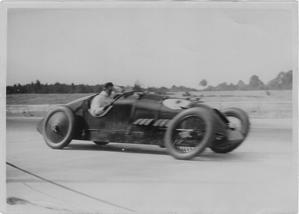
\includegraphics[scale=2.5]{./anamorphose.jpg}
 \scalebox{0.75}[0.75]{Photographie anamorphosée de Jacques Henri Lartigue}
\end{center}

\chapter{Compréhension théorique}
\underline{Problématique:} Comment simuler l'obturateur ?\bigskip

\noindent Solution: Parcourir la vidéo et récupérer une partie de chaque image pour créer l'image finale.
Chaque partie de l'image est une droite de pixel qui sera définie plus bas.\bigskip

\noindent Voici 4 idées de parcours de vidéo en fonction de l’action de l’utilisateur sur l’écran:\par\bigskip

1/Quatre parcours prédéfinis, les deux premiers en prenant des lignes verticales de pixels allant de droite à gauche ou de gauche à droite.
Les deux autres prenant des lignes horizontales de pixels allant de haut en bas ou de bas en haut (Annexe 4).
\begin{center}
 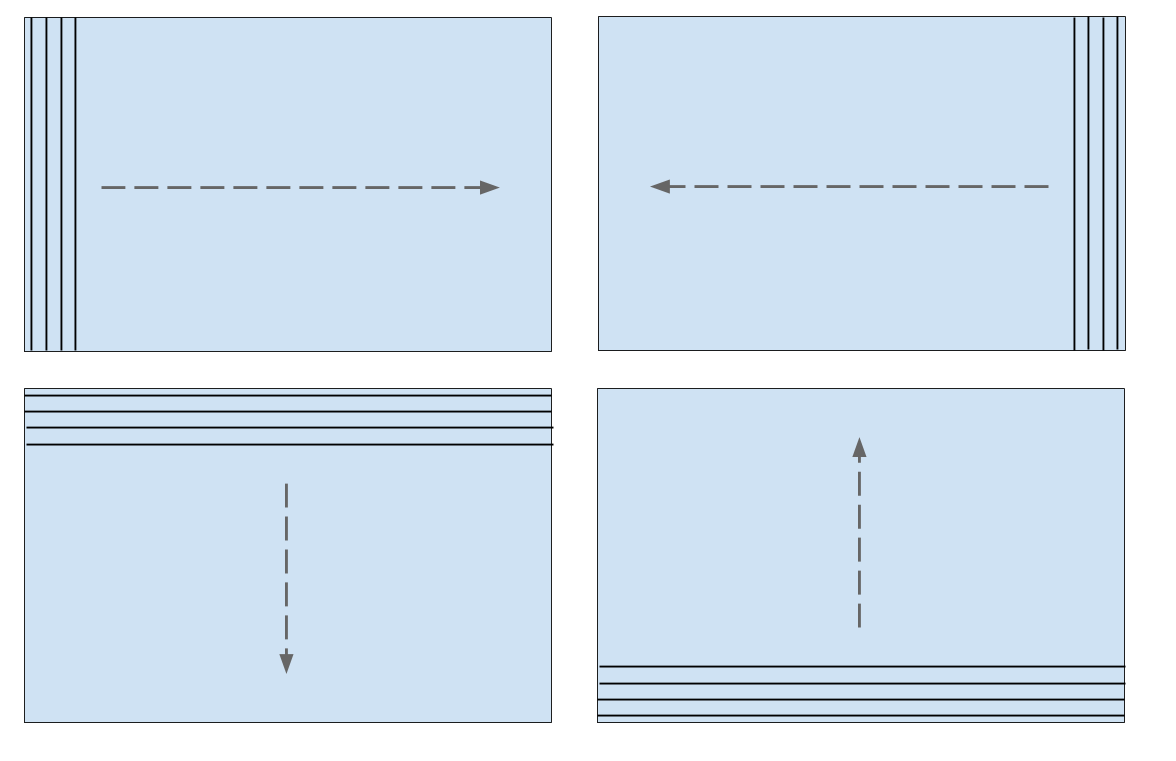
\includegraphics[scale=0.2]{./obturateur1.png}
\end{center}\newpage

2/ Un parcours linéaire suivant une direction et un sens personnalisé.
Pour cela on utilise un système de drag and drop, on pose le doigt sur l’écran en A(x1, y1), on reste appuyé sur l’écran en déplaçant son doigt et on relâche en B(x2, y2).
On obtient alors 2 points qui vont définir une direction et un sens de parcours.
On prendra alors dans chaque image, une droite perpendiculaire à la droite de parcours à une certaine position.
\begin{center}
 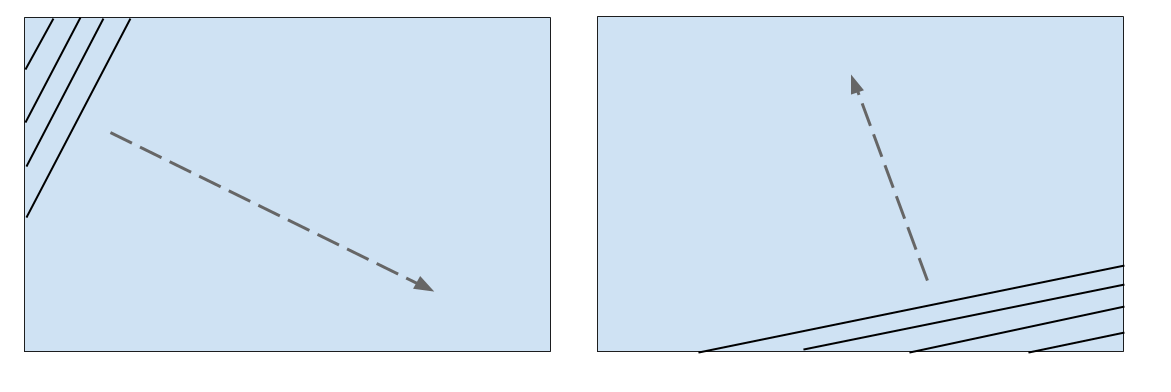
\includegraphics[scale=0.2]{./obturateur2.png}
\end{center}\par\bigskip

3/Un parcours personnalisé non linéaire (courbe) avec également un système de drag and drop. Pour un point, on prendra la perpendiculaire de la tangente en ce point.
On limitera cependant les déplacements pour éviter certains problèmes si l’utilisateur fait des mouvements compliqués.
Les déplacements pourront ainsi être faits selon ces différentes façon:
\\\indent -vers le haut et vers la droite
\\\indent -vers le haut et vers la gauche 
\\\indent -vers le bas et vers la droite
\\\indent -vers le bas et vers la gauche
\begin{center}
 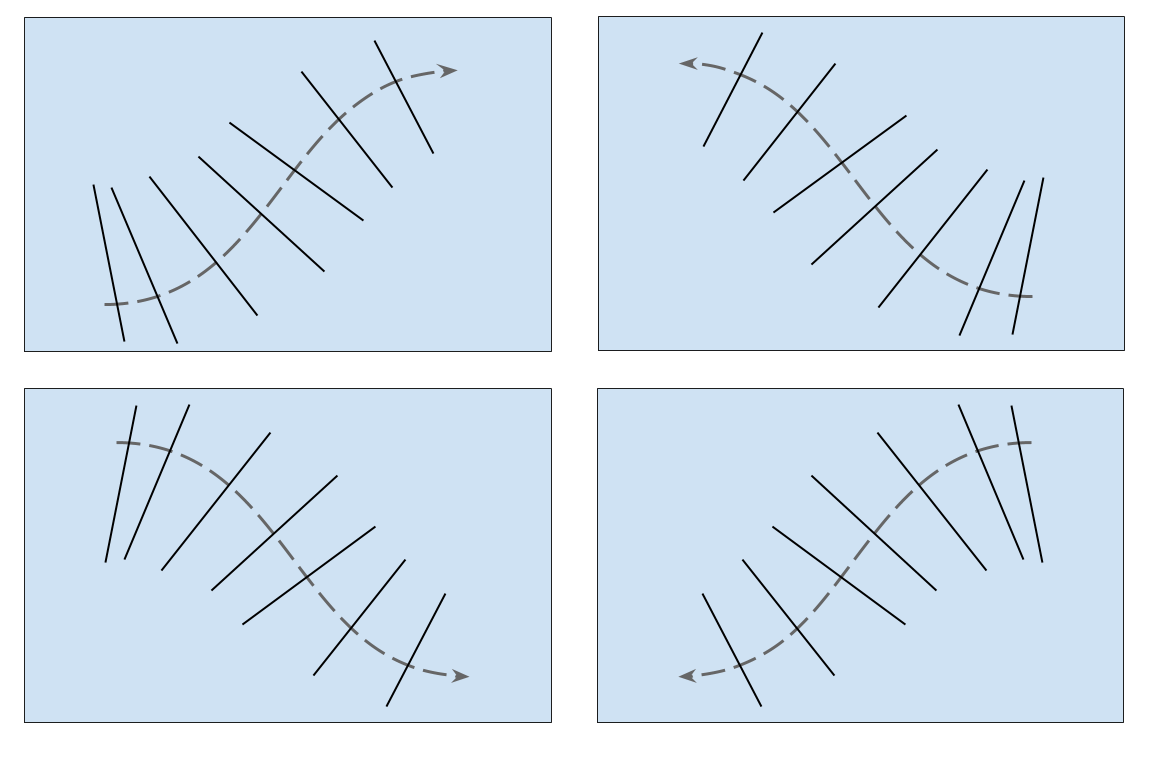
\includegraphics[scale=0.2]{./obturateur3.png}
\end{center}
On utilisera le critère suivant pour faire le remplissage entre 2 perpendiculaires :
\\\indent (1) On remplit tout ce qui est au dessus de toutes les précédentes perpendiculaires.
\\\indent (2) et out ce qui est en dessous de la perpendiculaire courante.
\begin{center}
 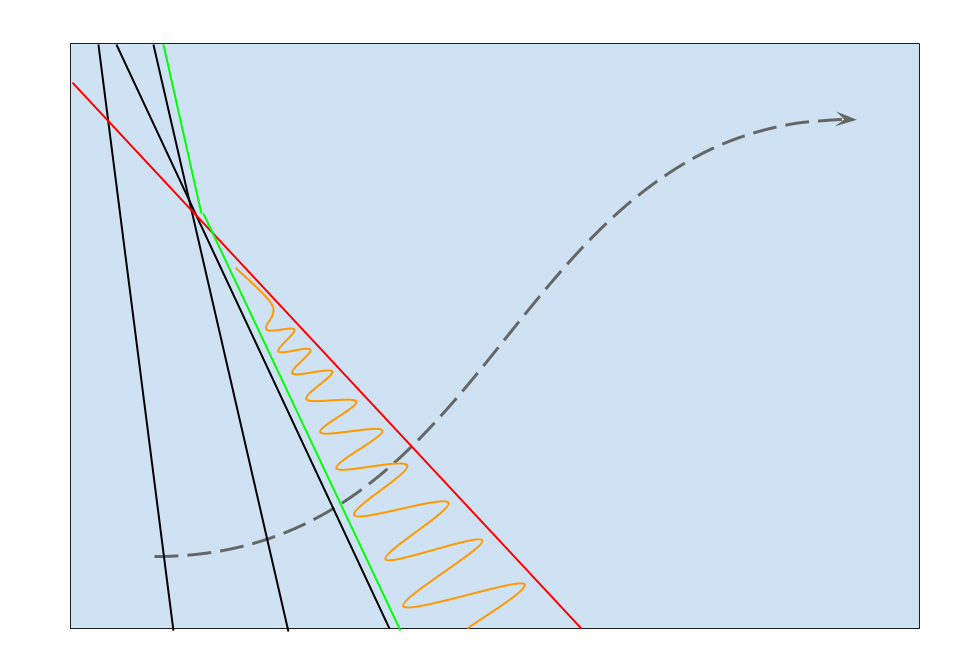
\includegraphics[scale=0.2]{./obturateur3exp.png}
\end{center}\par\bigskip
4/On ne limite pas les déplacements du doigt.
On limite alors les modifications de l’image finale à une zone restreinte centrée autour du point du calcul de la tangente.
\begin{center}
 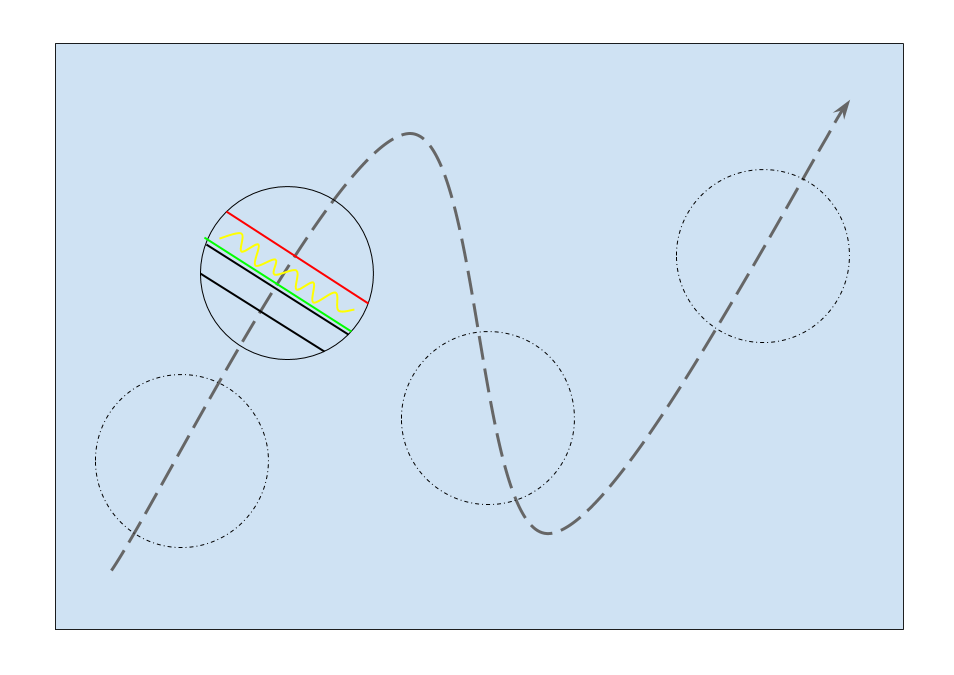
\includegraphics[scale=0.2]{./obturateur4.png}
\end{center}
Cette limitation est nécessaire car si on utilise les critères précédents (1) et (2),
il y aura des effets non voulus : remplacement de pixels en trop grande quantité, incertitude sur le calcul des segments au critère (1).
\begin{center}
 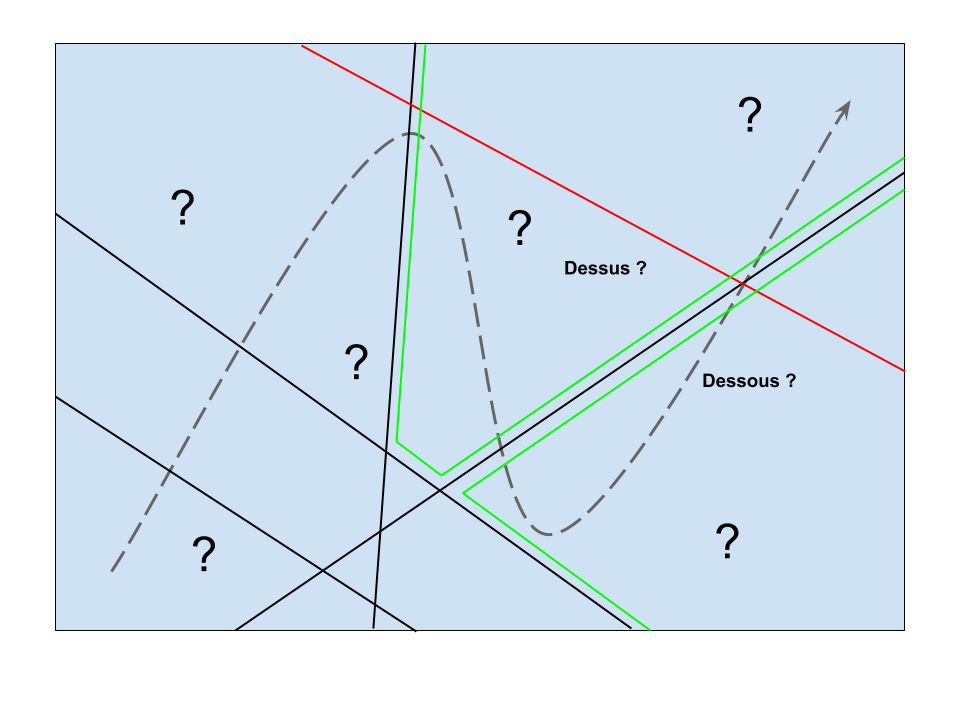
\includegraphics[scale=0.2]{./obturateur4exp.png}
\end{center}

\chapter{Travail réalisé}
En premier lieu, durant les deux premiers jours nous avons pris le temps de bien analyser et comprendre les subtilités du sujet. 
\\Nous avons tout d’abord fait une légère conception afin de cerner les besoins ainsi que les actions requises par l’utilisateur de notre application pour obtenir son image anamorphosée.
Ce brainstorming a résulté sur un diagramme de cas utilisateur (Annexe 1), un diagramme d’activité (Annexe 2) et un diagramme de séquence (Annexe 3) ainsi que des sketch de l’interface graphique.
\\Nous avons entamé des réflexions autour de l’algorithme à mettre en place et les différents problèmes qui pouvaient intervenir en fonction de certains certaines variables (forme de l’obturateur, tracé à suivre, etc).\bigskip

Dans un deuxième temps nous avons réfléchis à l’algorithme comme expliqué dans la section précédente.
Dans le même temps, une autre partie de l’équipe s’est attelé à la tâche consistant à récupérer toutes les frames d’une vidéo de façon la plus optimisée possible sur un smartphone android.
Après une recherche, plusieurs librairies comme OpenCV ou FFmepg  (https://github.com/wseemann/FFmpegMediaMetadataRetriever) nous fournissent les outils pour extraire des frames.
Cependant lors d’un premier test sur une vidéo de 6 secondes à 30fps cela prenait 56 secondes en moyenne pour extraires 90 frames.
Il paraissait donc évident qu’avec la capacité de nos téléphones actuelles, même avec plusieurs coeurs, cela prenait un temps considérable.
Il faudra ajouter à cela le traitement d’image a posteriori.
\\Après avoir threadé ce processus afin de le rendre plus rapide et moins bloquant (en terme d’interface utilisateur) le résultat fut le suivant: 50 secondes en moyenne pour extraire les 90 frames de la même vidéo.  Le constat n’est donc pas très concluant, en threadant le processus il n’y a pas un énorme gain et donc on peut prédire un problème de performances par la suite.

\newpage
La deuxième solution présentée dans la partie précédente a été testé avec la librairie Bitmap (en travaillant directement sur la hauteur et la largeur des images et non par rapport à leur matrice) fournie par Android,
le test a été fait assez rapidement, on a donc utilisé des fonctionnalités et des fonctions qui facilitent le test.
Cette solution est encore à étudier et ne sera pas forcément retenue.

\chapter{Travail à venir dans les prochains jours}
Après la recherche théorique et ayant une idée bien plus précise et réfléchi de l’algorithme qui a été écrit en java, nous devons dorénavant l’implémenter avec
les spécifications d’android (avec la classe Bitmap pour créer une image à partir d’une matrice par exemple) afin de le tester en pratique et vérifier son bon fonctionnement ainsi que ses performances.

\chapter{Annexes}
\section{UseCase}
\begin{center}
 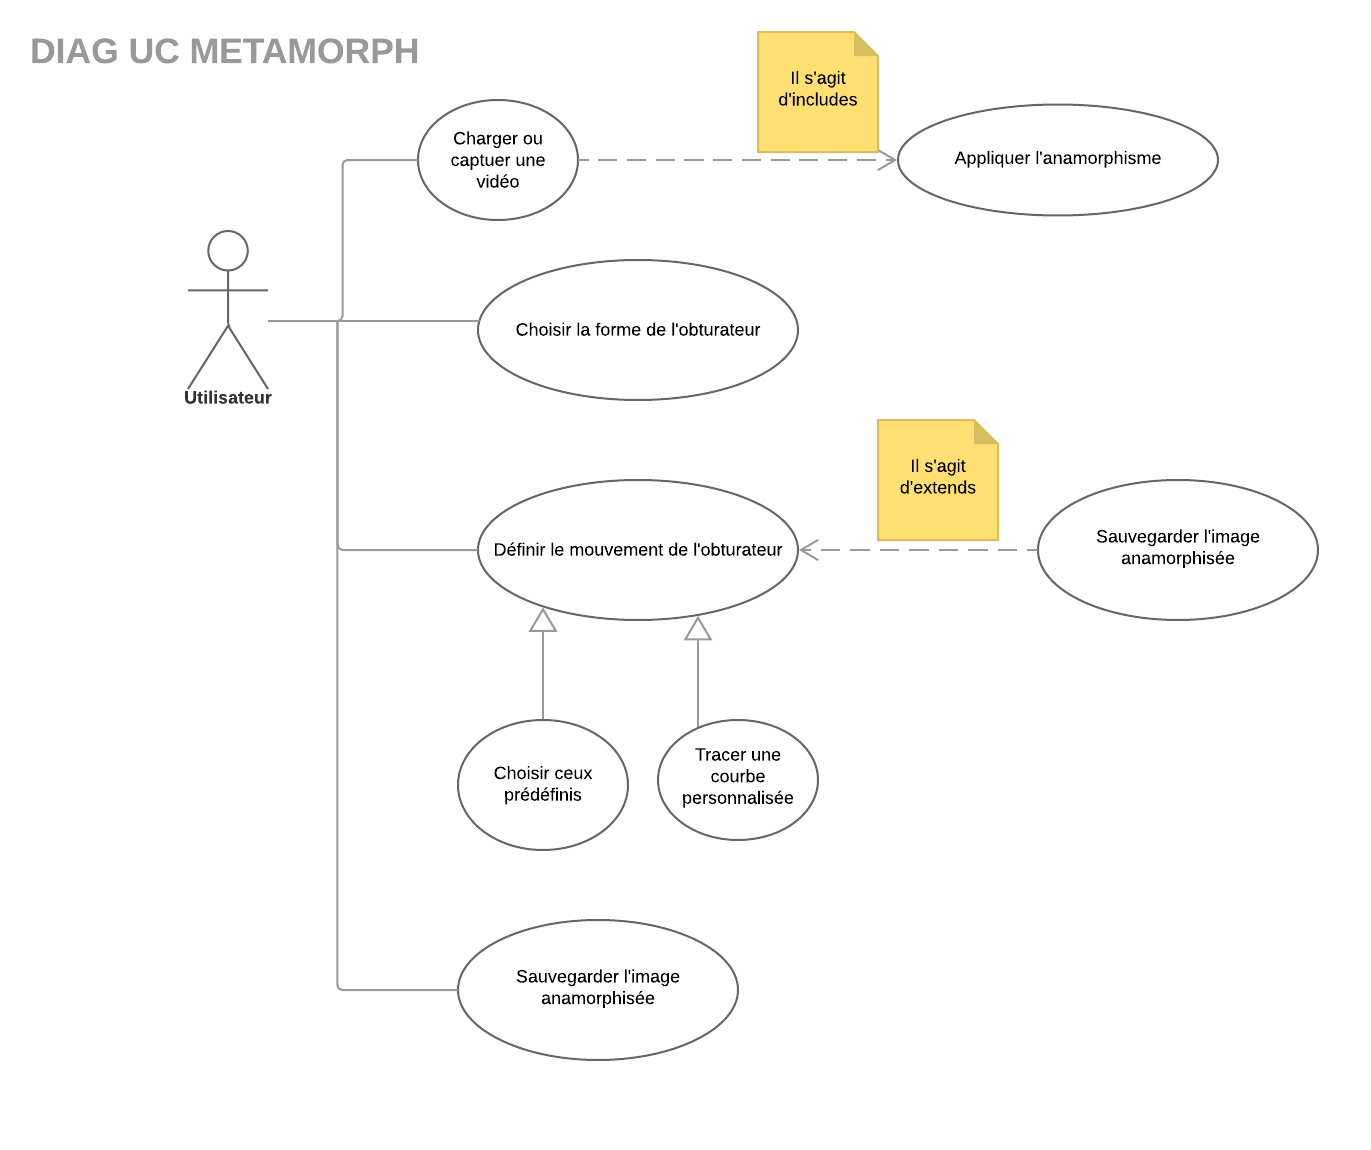
\includegraphics[scale=0.65]{./UC.png}
\end{center}

\section{Activity}
\begin{center}
 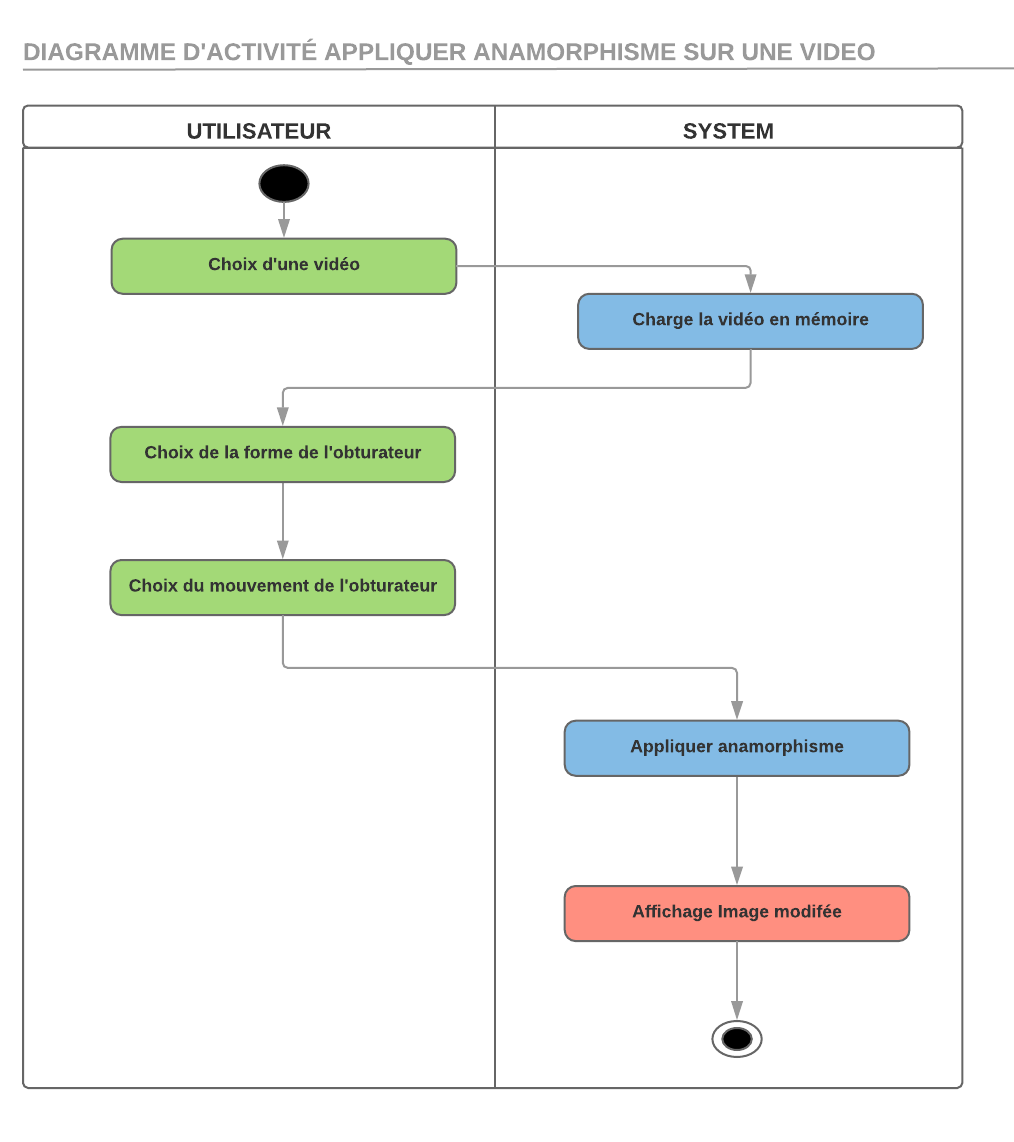
\includegraphics[scale=0.7]{./Activites.png}
\end{center}

\section{Sequence}
\begin{center}
 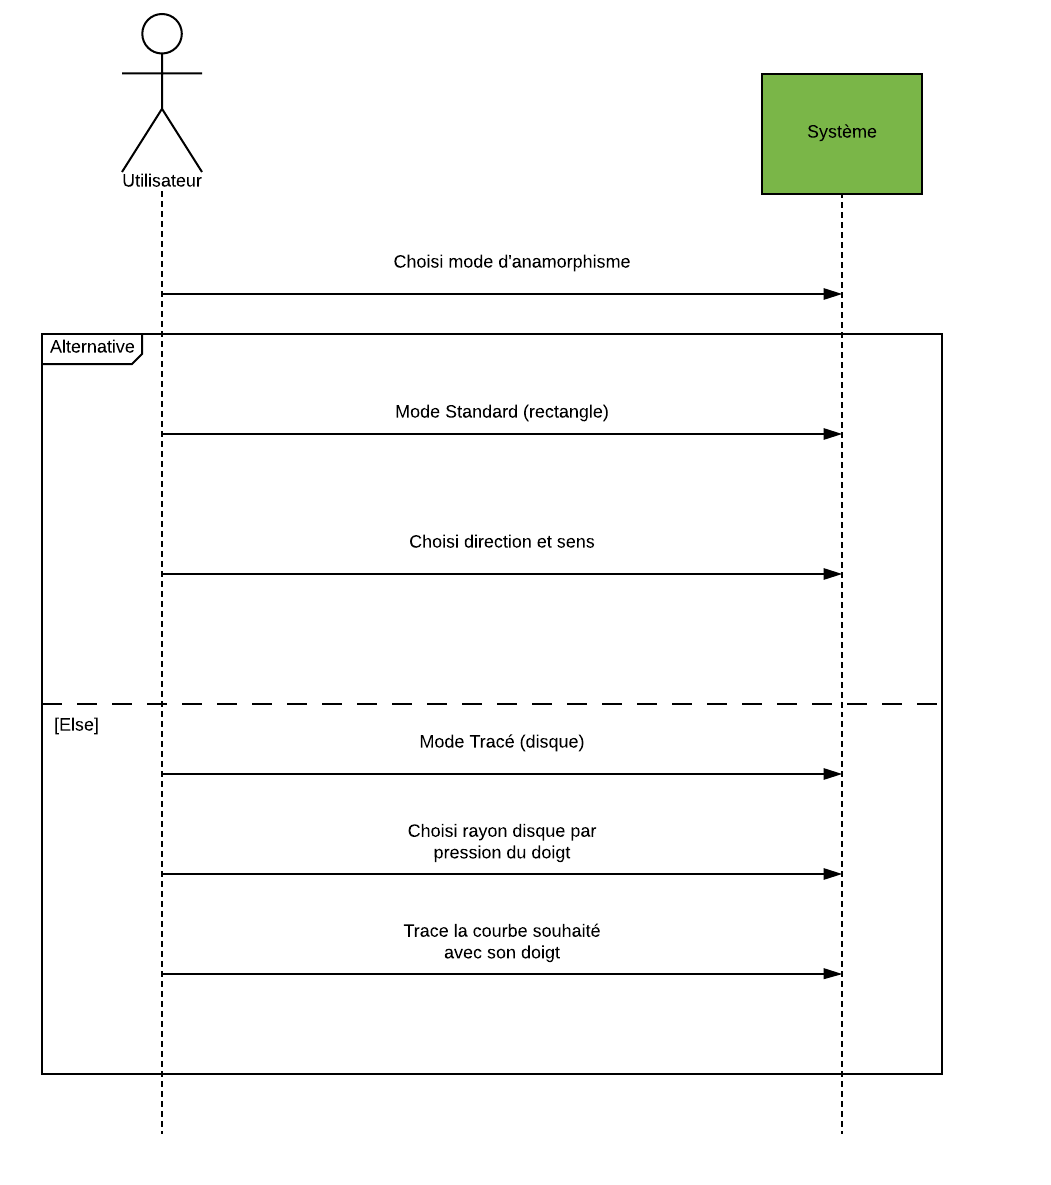
\includegraphics[scale=0.7]{./Sequence.png}
\end{center}
\newpage
\section{Algorithme avec déplacement simple de l'obturateur}
\begin{verbatim}
liste_img : liste des images (on suppose qu’une image est un tableau à 
	    2 dimensions, chaque élément est un pixel)
N : nombre d’images dans la liste des images
l : longueur des images
h : hauteur des images
img : image finale anamorphosée
s1 : systeme 1
s2 : systeme 2
s3 : systeme 3
\end{verbatim}

\noindent\textbf{Retourne:} img \bigskip

\noindent\textbf{\underline{Explications:}}
\begin{verbatim}
A chaque tour de boucle, on saute (s1) lignes.
Tous les (s3) tours de boucle, on saute une ligne

    Ex: Pour un algo de sens vertical, soit N = 10 et h = 4
        On calcul alors s1 = 2, s3 = 2
        A chaque tour de boucle, on saute (2) lignes.
Tous les (2) tours de boucle, on saute une ligne.
En suivant ce schéma, on arrive a utiliser les images de la vidéo de manière.
à ce qu’elles soient équitablement prises dans la liste,
ie : les saut sont répartis un peu partout dans la liste.


On écrit 4 algos pour être le plus performant.
\end{verbatim}
\newpage
\noindent\textbf{haut vers bas et bas vers haut (partie commune):}
\begin{verbatim}
s1 = N/h
s2 = N%h
if s2 !=0
s3 = h/s2
else
    s3 = h+1 // pour ne jamais remplir la condition du if

\end{verbatim}
\bigskip
\noindent\textbf{haut vers bas:}
\begin{verbatim}
saut = s3
cpt = 0
for i in (0, h):  // pour chaque ligne de l’image finale
    if i > saut:
        cpt ++
        saut += s3
    for j in (0, l): // pour chaque element dans la ligne
        img[i][j] = liste_img[cpt][i][j]
    cpt += s1

\end{verbatim}
\bigskip
\noindent\textbf{bas vers haut:}
\begin{verbatim}
saut = s3
cpt = 0
for i in (0, h):  // pour chaque ligne de l’image finale
    if i > saut:
        cpt ++
        saut += s3
    for j in (0, l): // pour chaque element dans la ligne
        img[i][ j] = liste_img[cpt][h-1-i][j]
    cpt += s1

\end{verbatim}
\newpage
\noindent\textbf{gauche vers droite et droite vers gauche (partie commune):}
\begin{verbatim}
s1 = N/l   
s2 = N%l
if s2 !=0
s3 = l/s2
else
    s3 = l+1 // pour ne jamais remplir la condition du if

\end{verbatim}
\bigskip
\noindent\textbf{gauche vers droite:}
\begin{verbatim}
saut = s3
cpt = 0
for j in (0, l):  // pour chaque colonne de l’image finale
    if j > saut:
        cpt ++
        saut += s3
    for i in (0, h): // pour chaque element dans la colonne
        img[j][i] = liste_img[cpt][j][i]
    cpt += s1

\end{verbatim}
\bigskip
\noindent\textbf{droite vers gauche:}
\begin{verbatim}
saut = s3
cpt = 0
for j in (0, l):  // pour chaque ligne de l’image finale
    if j > saut:
        cpt ++
        saut += s3
    for i in (0, h): // pour chaque element dans la ligne
        img[i][j] = liste_img[cpt][i][l-1-j]
    cpt += s1
\end{verbatim}



\end{document}
